\begin{frame}
\frametitle{Participate!}
During the lectures...
\begin{itemize}
\item Don't hesitate to ask questions. Other people in the audience may have
similar questions too.
\item This helps the trainer to detect any explanation that wasn't clear or
detailed enough.
\item Don't hesitate to share your experience, for example to compare Linux
with other operating systems used in your company.
\item Your point of view is most valuable, because it can be similar to your
colleagues' and different from the trainer's.
\item Your participation can make our session more interactive and make the
topics easier to learn.
\end{itemize}
\end{frame}

\section{Base Theory and Concepts About Graphics}

\subsection{Image and Color Representation}

\begin{frame}{Light, pixels and pictures}
  \begin{minipage}{0.75\textwidth}
  \begin{itemize}
  \item Pictures are {\bf representations of light emissions}
  \item Analog representations are spatially {\bf continuous}:
    \begin{itemize}
    \item With an {\bf infinite} number of elements
    \item Example : photosensitive paper
    \end{itemize}
  \item Digital representations are spatially {\bf quantified}:
    \begin{itemize}
    \item With a {\bf finite} number of elements
    \item Example : discrete LED-based display
    \end{itemize}
  \item Producing a digital representation is called \textbf{quantization}
    \begin{itemize}
    \item Reduction of information from the continuous world
    \item Quantization requires a {\bf base element unit} or quantum
    \item This quantum is called picture element or {\bf pixel}
    \item Quantization is also called \textbf{sampling} in this context
    \end{itemize}
  \end{itemize}
  \end{minipage}%
  \begin{minipage}{0.25\textwidth}
  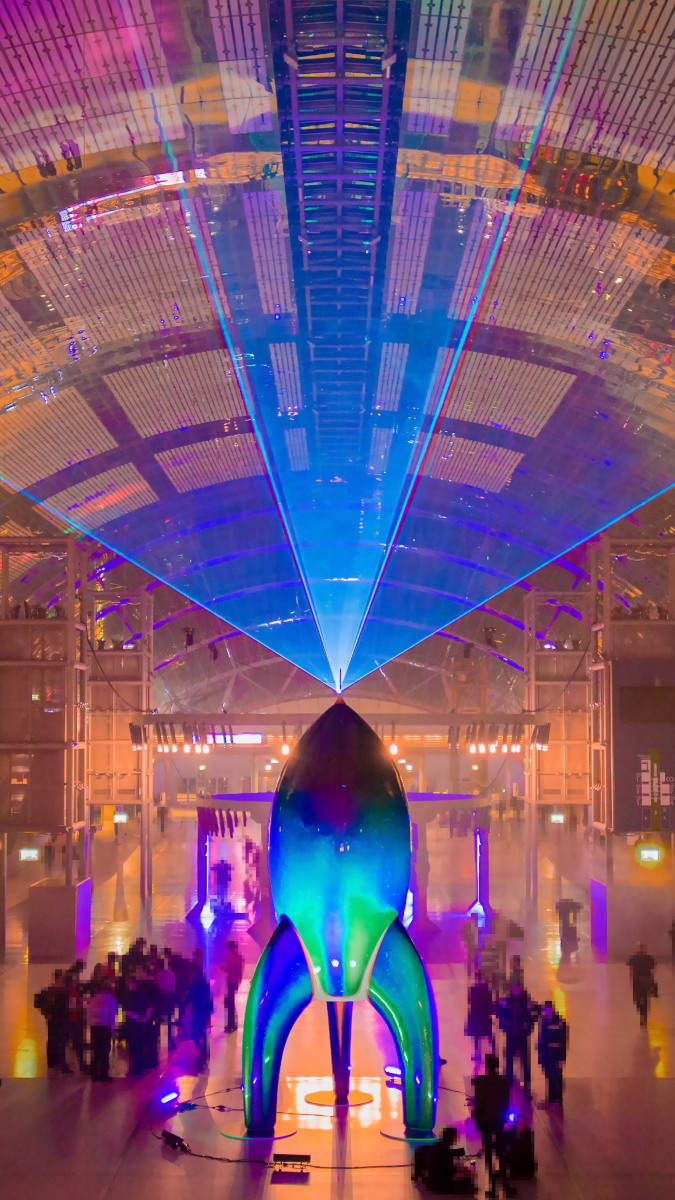
\includegraphics[width=\textwidth]{slides/graphics-theory/ccc-rocket.jpg}
  \end{minipage}
\end{frame}

\begin{frame}{Light, pixels and pictures}
  \begin{itemize}
  \item \textbf{Pictures} are bi-dimensional ordered ensembles of pixels (also called \textbf{frames}):
    \begin{itemize}
    \item Frames have \textbf{dimensions}: \textbf{width} (horizontal) and \textbf{height} (vertical)
    \item The aspect ratio is the \textbf{width:height} ratio (e.g. 16:9, 4:3)
    \item Pixels are located with a \textbf{position}: \textbf{(x,y)}
    \item The dimension and position unit is the number of pixels
    \end{itemize}
  \item Quantified pixels have a \textbf{spatial density} or spatial resolution:\\
    \begin{itemize}
    \item \textit{How many pixels are found in \(n\) inches?}
    \item The usual pixel resolution unit is the \textbf{dot per inch} (DPI)
    \item Vertical and horizontal spatial densities are usually not distinguished\\
      \textit{pixels are assumed to have a square shape most of the time}
    \end{itemize}
  \end{itemize}

\end{frame}

\begin{frame}{Light, pixels and pictures (illustrated)}
  \begin{minipage}[b]{0.45\textwidth}
    \centering
    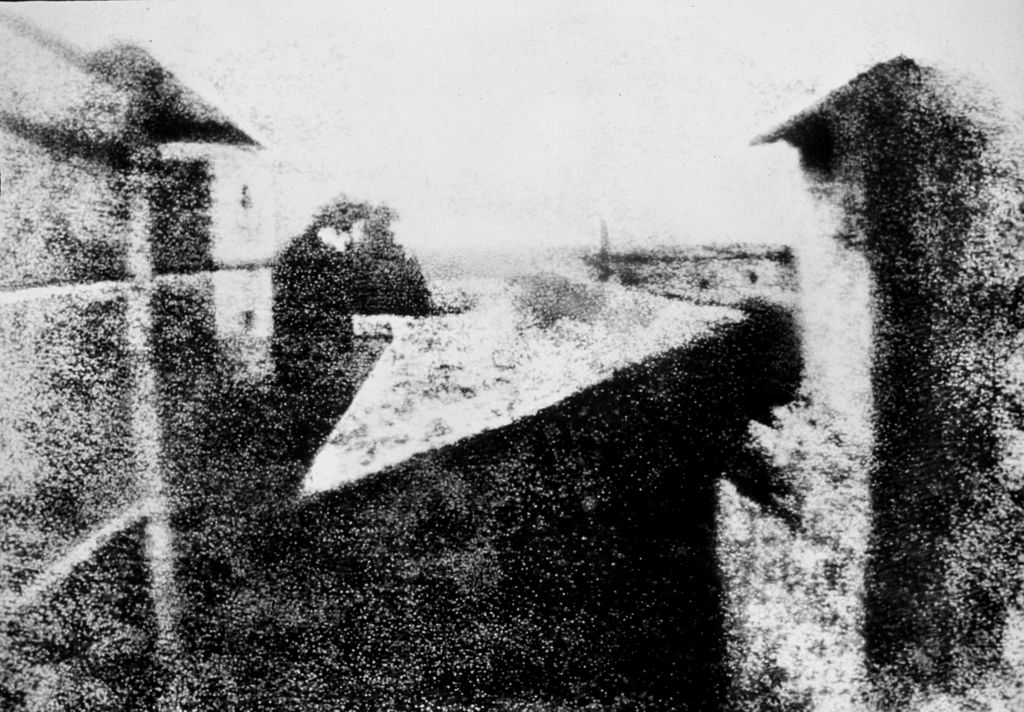
\includegraphics[width=\textwidth]{slides/graphics-theory/first-photo.jpg}
    \textit{\small View from the Window at Le Gras picture}
  \end{minipage}
  \hfill
  \begin{minipage}[b]{0.45\textwidth}
    \centering
    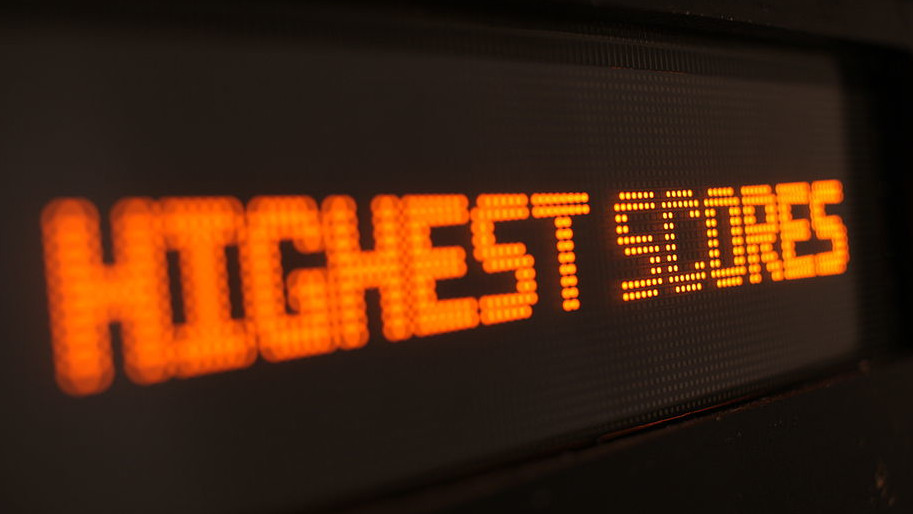
\includegraphics[width=\textwidth]{slides/graphics-theory/dot-matrix-display.jpg}
    \textit{\small A monochrome dot-matrix display}
  \end{minipage}

  \vspace{1em}

  \begin{minipage}[b]{0.45\textwidth}
    \centering
    \textbf{Analog representation},\\ on a metal plate
  \end{minipage}
  \hfill
  \begin{minipage}[b]{0.45\textwidth}
    \centering
    \textbf{Digital representation},\\ on a LED display
  \end{minipage}
\end{frame}

\begin{frame}{Sampling and frequency domain}
  \begin{itemize}
  \item Pixels are quantized/sampled representations of a \textbf{spatial domain}
  \item The initial (continuous) domain has a corresponding \textbf{frequency spectrum}\\
    \textit{high frequencies provide details in pictures}
  \item A 2D \textbf{Fourier transform} translates from spatial \((x,y)\) to frequency \((u,v)\) domain
\[
F(u,v) = \int_{-\infty}^{+\infty} \int_{-\infty}^{+\infty} f(x,y)e^{-j2\pi(ux+uy)}dxdy
\]
  \item The transform decomposes the domain in \textbf{periodic patterns}
  \item Adapted for discrete signals as \textbf{Discrete Fourier Transform}
  \item Implemented with optimized algorithms as \textbf{Fast Fourier Transform} (FFT)
  \item \textbf{Frequency domain analysis} is very useful for signal processing\\
    \textit{used at the roots of image compression}
  \end{itemize}
\end{frame}

\begin{frame}{Sampling and frequency domain (illustrated)}
  \begin{center}
  \begin{minipage}[b]{0.45\textwidth}
    \centering
    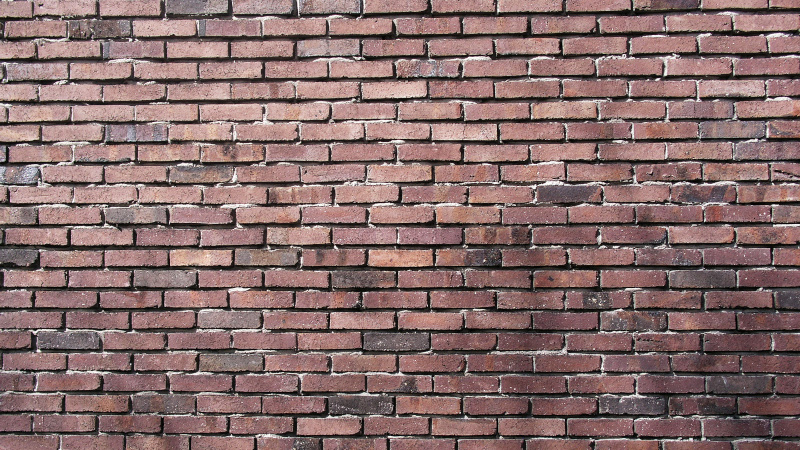
\includegraphics[width=\textwidth]{slides/graphics-theory/bricks.jpg}\\
    \textit{\small A wall of bricks represented in the spatial domain}
  \end{minipage}
  \hfill
  \begin{minipage}[b]{0.45\textwidth}
    \centering
    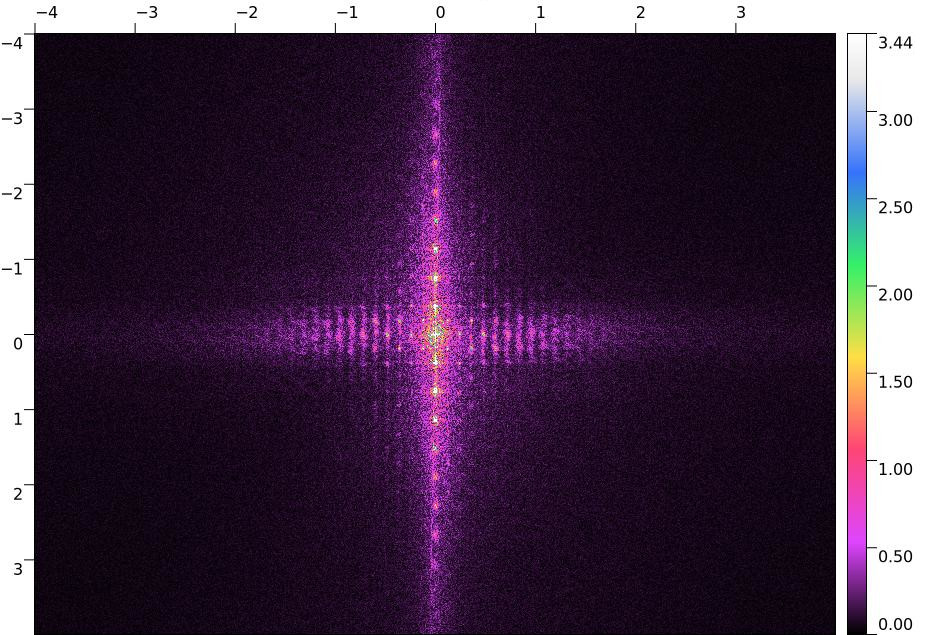
\includegraphics[width=\textwidth]{slides/graphics-theory/bricks-fft.jpg}\\
    \textit{\small The wall of bricks represented in the frequency domain}
  \end{minipage}

  \end{center}
\end{frame}

\begin{frame}{Sampling and frequency domain (illustrated)}
  \begin{minipage}[b]{0.45\textwidth}
    \centering
    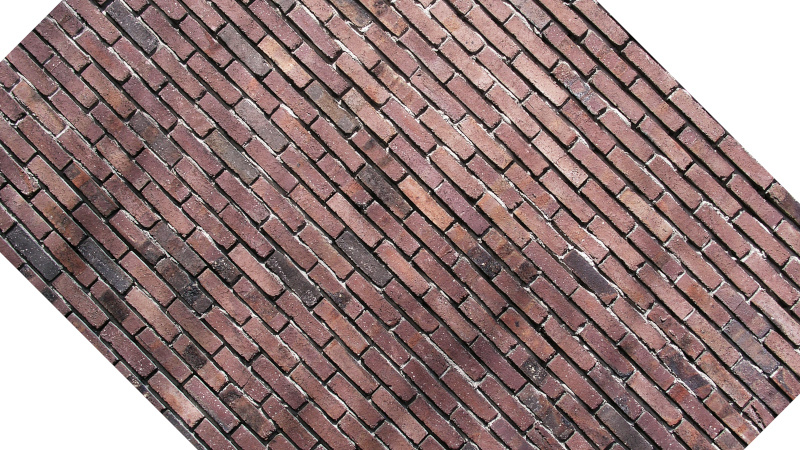
\includegraphics[width=\textwidth]{slides/graphics-theory/bricks-rotation.jpg}\\
    \textit{\small A wall of bricks rotated \(45^{\circ}\) represented in the spatial domain}
  \end{minipage}
  \hfill
  \begin{minipage}[b]{0.45\textwidth}
    \centering
    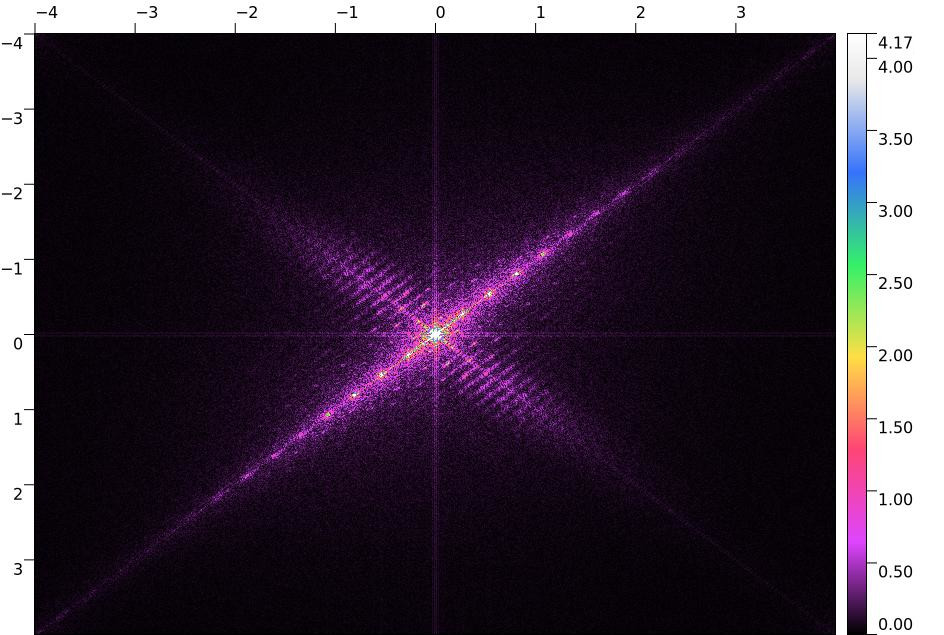
\includegraphics[width=\textwidth]{slides/graphics-theory/bricks-fft-rotation.jpg}\\
    \textit{\small The wall of bricks rotated \(45^{\circ}\) represented in the frequency domain}
  \end{minipage}
\end{frame}

\begin{frame}{Sampling and aliasing}
  \begin{itemize}
  \item The spatial domain is quantized with a bi-dimensional \textbf{sampling resolution}
  \item Matching \textbf{sampling frequencies} exist, for each axis: \((u_s,v_s)\)
  \item They \textbf{limit the frequencies} that can be sampled from the initial domain
  \item The \textbf{Shannon-Nyquist theorem} provides a sufficient condition for \((u_s,v_s)\):
\[
u_s > 2 \times u_{max}, ~v_s > 2 \times v_{max}
\]
  \item Frequencies such that \(f \geq \frac{f_s}{2}\) are \textbf{not correctly sampled}
  \item Can result in \textbf{incorrect frequencies} being introduced: \textbf{Moiré pattern} in 2D
  \end{itemize}

  \begin{center}
  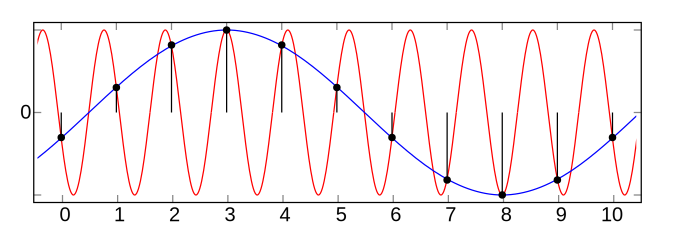
\includegraphics[width=0.35\textwidth]{slides/graphics-theory/aliasing-1d.pdf}\\
  \textit{\small Aliasing example in a uni-dimensional domain}
  \end{center}
\end{frame}

\begin{frame}{Sampling and aliasing (illustrated)}
  \begin{minipage}[b]{0.29\textwidth}
    \centering
    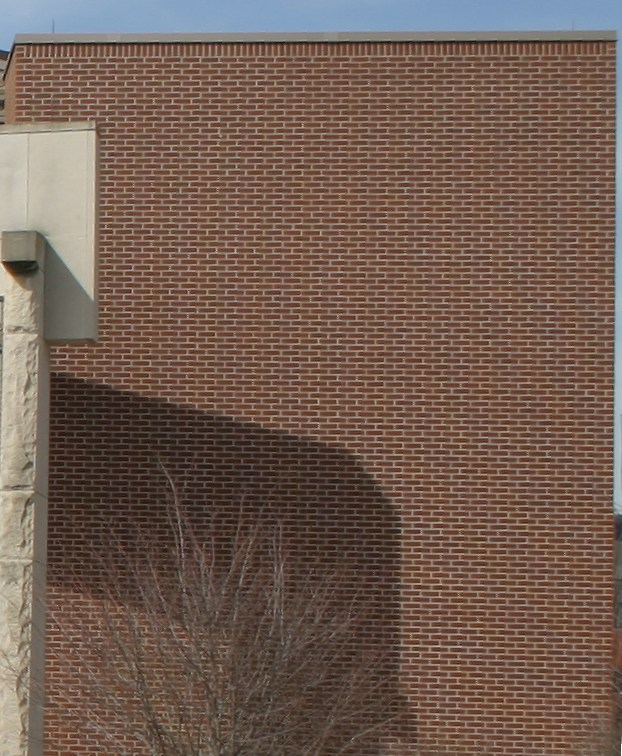
\includegraphics[width=\textwidth]{slides/graphics-theory/bricks-rich.jpg}\\
    \textit{\small Another wall of bricks}
  \end{minipage}
  \hfill
  \begin{minipage}[b]{0.29\textwidth}
    \centering
    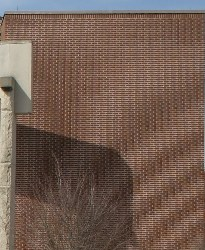
\includegraphics[width=\textwidth]{slides/graphics-theory/bricks-alias.jpg}\\
    \textit{\small Moiré on the bricks}
  \end{minipage}
  \hfill
  \begin{minipage}[b]{0.29\textwidth}
    \centering
    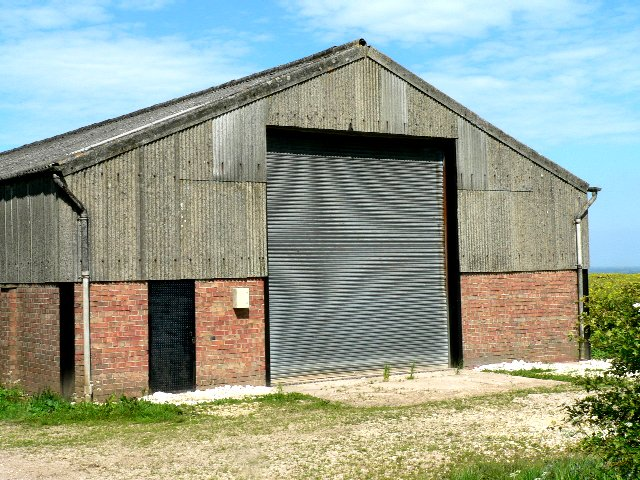
\includegraphics[width=\textwidth]{slides/graphics-theory/moire.jpg}\\
    \textit{\small Moiré on the garage door}
  \end{minipage}
\end{frame}

\begin{frame}{Light representation, color quantization}
  \begin{minipage}[c]{0.75\textwidth}
    \begin{itemize}
    \item \textbf{Light} itself must be quantized in digital representations\\
    \textit{distinct from and unrelated to spatial quantization}
    \item \textbf{Translating} light information (colors) to numbers:
      \begin{itemize}
      \item Using a translation referential called \textbf{colorspace}
      \item The translated color has \textbf{coordinates} in the colorspace\\
      \textit{e.g. 3 for a human-eye-alike referential: red, green, blue}
      \end{itemize}
    \item Color coordinates are quantized with:
      \begin{itemize}
      \item A given \textbf{resolution}:
      \textit{the smallest possible color difference}
      \item A given \textbf{range}:
      \textit{the span of representable colors}
      \end{itemize}
    \item Different approaches exist for color quantization:
      \begin{itemize}
      \item \textbf{Uniform} quantization in the color range (most common)\\
        \textit{values are attributed to colors with a regular step (resolution)}
      \item \textbf{Irregular} quantization with indexed colors (palettes)\\
        \textit{values are attributed to colors as needed}
      \end{itemize}
    \end{itemize}
  \end{minipage}
  \hfill
  \begin{minipage}[c]{0.225\textwidth}
    \centering
    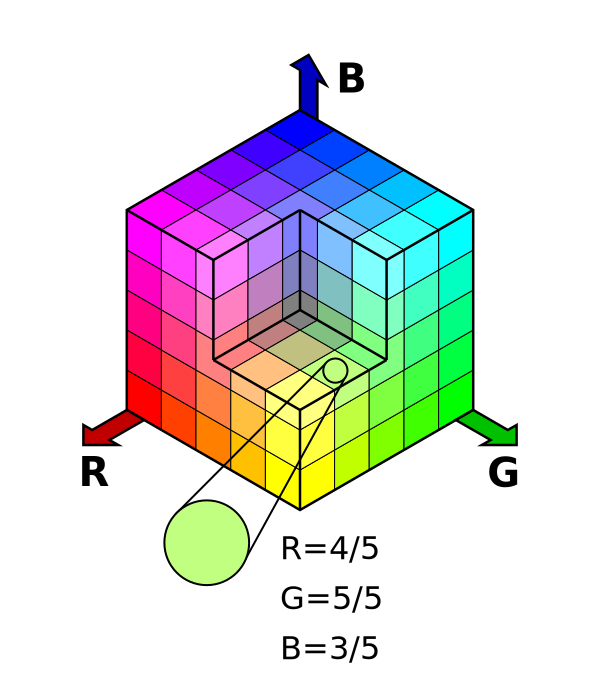
\includegraphics[width=\textwidth]{slides/graphics-theory/rgb-cube.pdf}
  \end{minipage}
\end{frame}

\begin{frame}{Light representation, color quantization (illustrated)}
  \begin{minipage}[b]{0.45\textwidth}
    \centering
    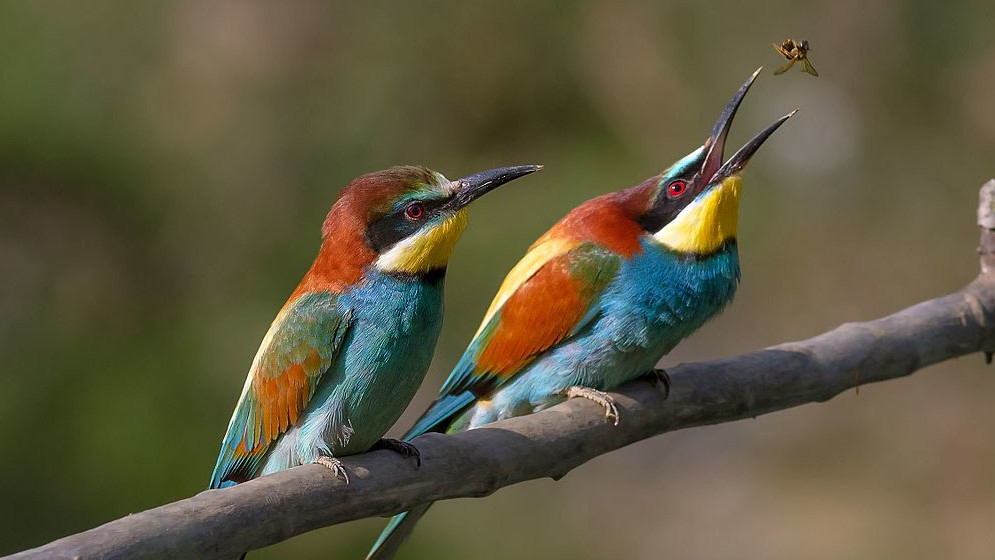
\includegraphics[width=\textwidth]{slides/graphics-theory/pair-of-merops.jpg}
  \end{minipage}
  \hfill
  \begin{minipage}[b]{0.45\textwidth}
    \centering
    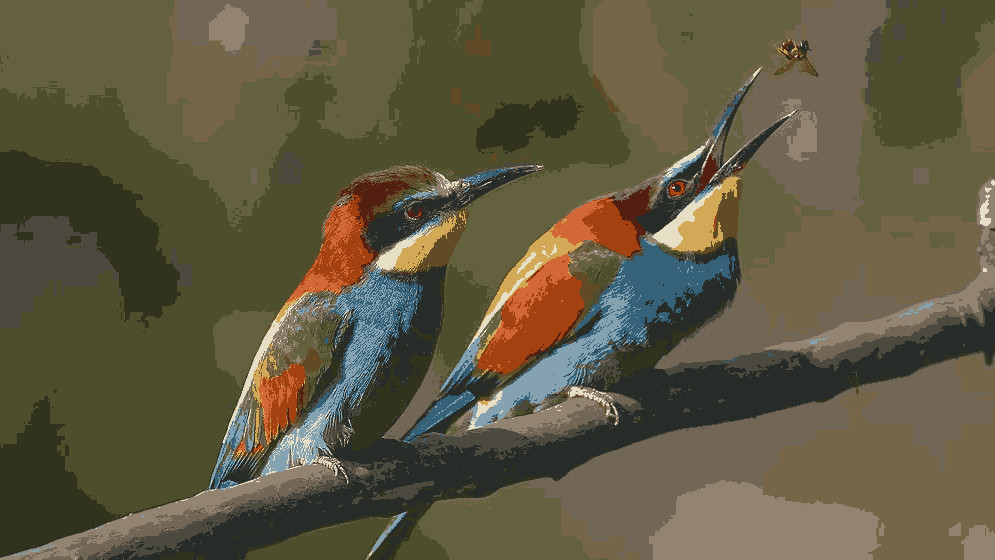
\includegraphics[width=\textwidth]{slides/graphics-theory/pair-of-merops-16-colors.jpg}
  \end{minipage}

  \begin{center}
     \textit{\small A pair of Merops feeding}
  \end{center}

  \begin{minipage}[b]{0.45\textwidth}
    \centering
    \textbf{16 million colors (24 bits per pixel)}
    \begin{itemize}
    \item high color resolution
    \item high color range
    \end{itemize}
  \end{minipage}
  \hfill
  \begin{minipage}[b]{0.45\textwidth}
    \centering
    \textbf{16 colors (4 bits per pixel)}
    \begin{itemize}
    \item low color resolution
    \item low color range
    \end{itemize}
  \end{minipage}
\end{frame}

\begin{frame}{Light representation, color quantization (illustrated)}
  \begin{minipage}[b]{0.45\textwidth}
    \centering
    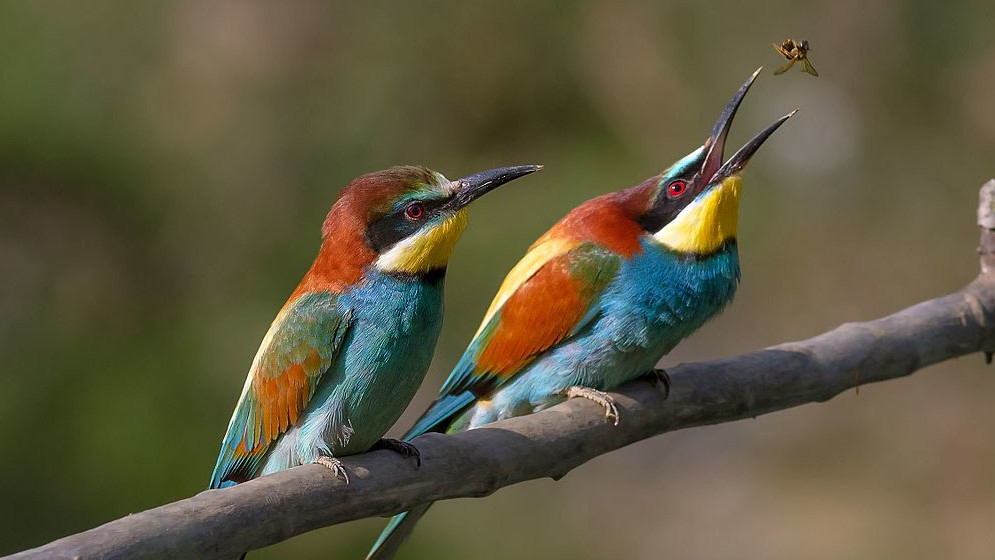
\includegraphics[width=\textwidth]{slides/graphics-theory/pair-of-merops.jpg}
  \end{minipage}
  \hfill
  \begin{minipage}[b]{0.45\textwidth}
    \centering
    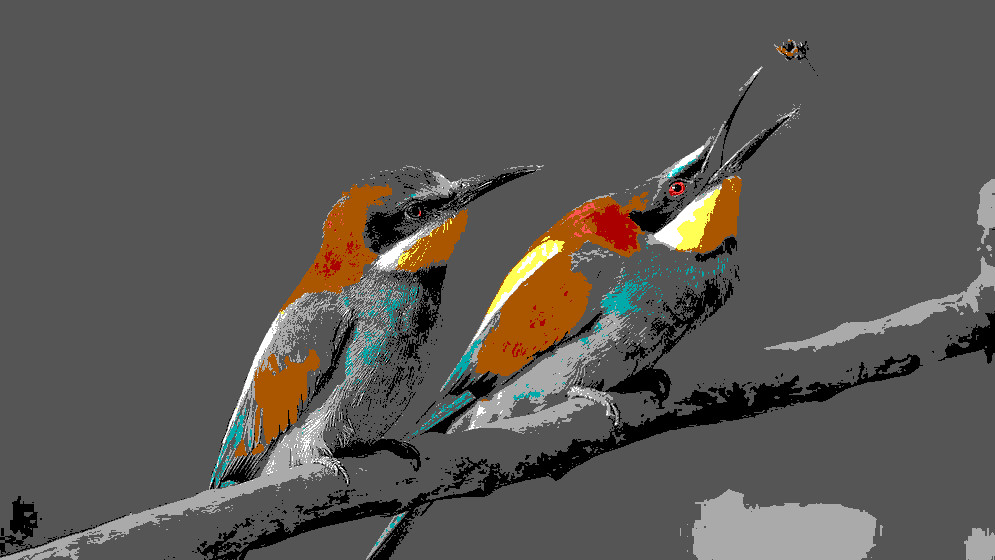
\includegraphics[width=\textwidth]{slides/graphics-theory/pair-of-merops-16-colors-range.jpg}
  \end{minipage}

  \begin{center}
     \textit{\small A pair of Merops feeding}
  \end{center}

  \begin{minipage}[b]{0.45\textwidth}
    \centering
    \textbf{16 million colors (24 bits per pixel)}
    \begin{itemize}
    \item high color resolution
    \item high color range
    \end{itemize}
  \end{minipage}
  \hfill
  \begin{minipage}[b]{0.45\textwidth}
    \centering
    \textbf{16 colors (4 bits per pixel)}
    \begin{itemize}
    \item lower color resolution
    \item high color range
    \end{itemize}
  \end{minipage}
\end{frame}

\begin{frame}{Colorspaces and channels}
  \begin{minipage}[b]{0.7\textwidth}
    \begin{itemize}
    \item Each component of a colorspace is called a \textbf{channel}
    \item Examples for usual types of colorspaces:
      \begin{itemize}
      \item RGB, with 3 channels:\\ \textbf{R} (red) / \textbf{G} (green) / \textbf{B} (blue)
      \item HSV, with 3 channels:\\ \textbf{H} (hue) / \textbf{S} (saturation) / \textbf{V} (value)
      \item YUV or Y/Cb/Cr, with 3 channels:\\ \textbf{Y} (luminance) / \textbf{U or Cb} / \textbf{V or Cr} (chrominance)
      \end{itemize}
    \end{itemize}
  \end{minipage}
  \hfill
  \begin{minipage}[b]{0.25\textwidth}
    \centering
    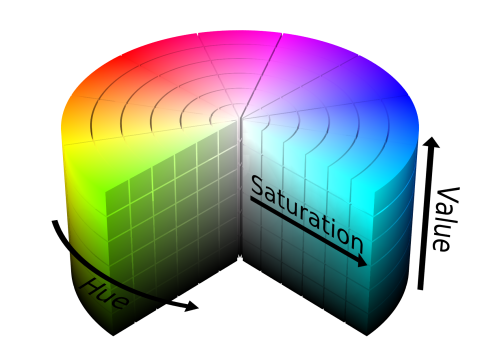
\includegraphics[width=\textwidth]{slides/graphics-theory/hsv-diagram.pdf}\\
    \vspace{-1em}
    \textit{\small HSV diagram}
    \vspace{0.25em}
  \end{minipage}
  \begin{itemize}
  \item An additional channel can exist for transparency: the \textbf{alpha channel}\\
  \textit{mostly relevant for composition, not for final display}
  \item Color coordinates can be \textbf{converted} from one colorspace to another (CSC)\\
  \textit{using translation formulas and associated constants}
  \end{itemize}
\end{frame}

\begin{frame}{Colorspaces and channels (illustrated with YUV)}
  \begin{minipage}[t]{0.25\textwidth}
    \centering
    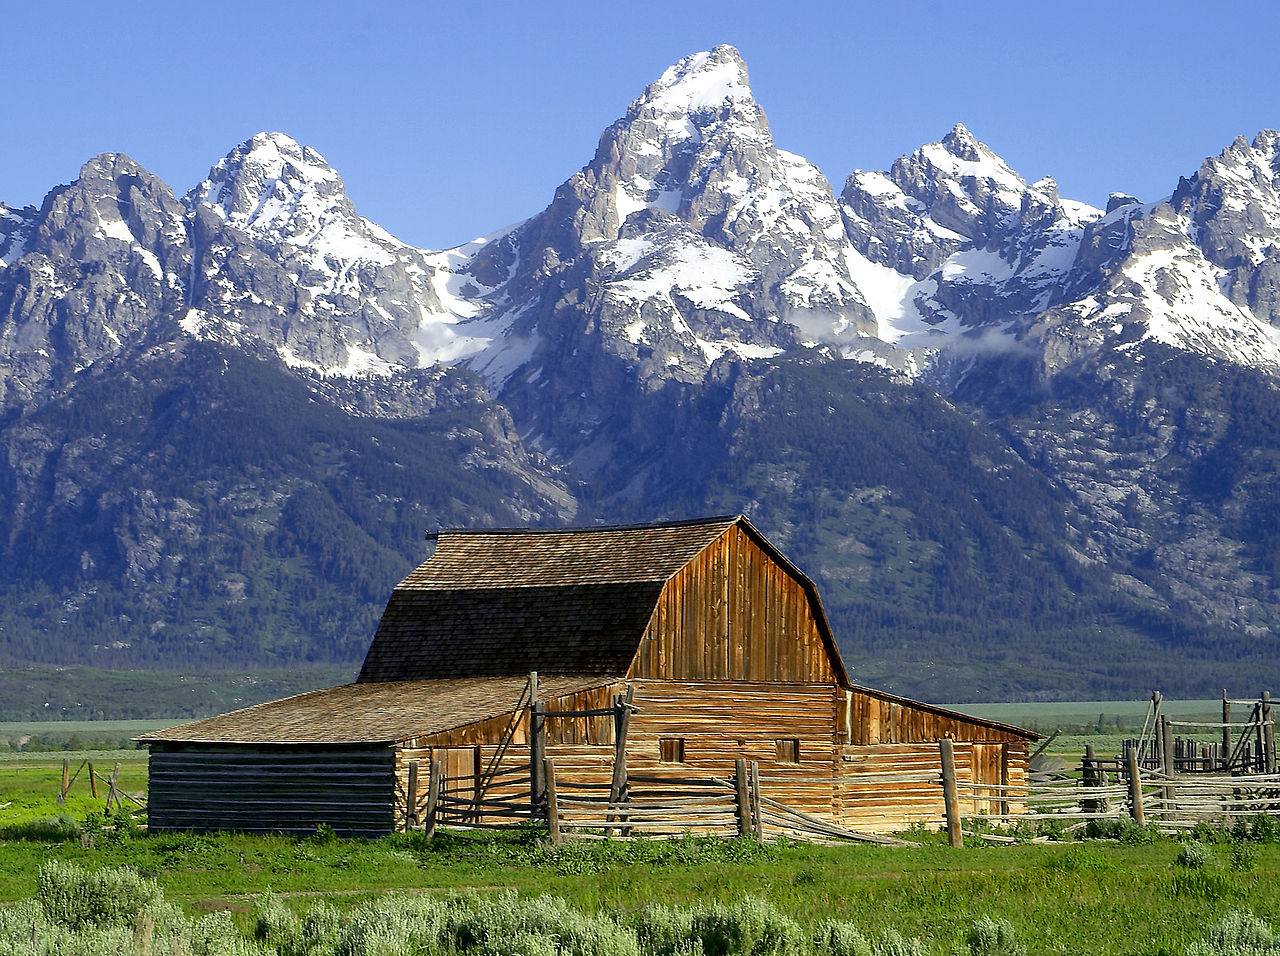
\includegraphics[height=6em]{slides/graphics-theory/barn.jpg}\\
    \textit{\small Original picture}
  \end{minipage}
  \hfill
  \begin{minipage}[t]{0.7\textwidth}
    \centering
    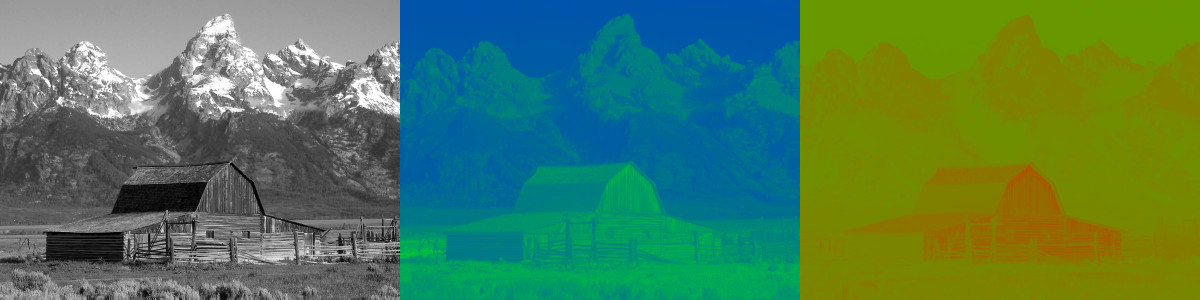
\includegraphics[height=6em]{slides/graphics-theory/barn-yuv.jpg}\\
    \textit{\small Decomposition in Y, U and V channels}
  \end{minipage}

  \vspace{1em}

  \begin{minipage}[t]{0.4\textwidth}
    \small
    \begin{equation*}
    \begin{cases}
    R = Y + 1.140 \times V\\
    G = Y - 0.395 \times U - 0.581 \times V\\
    B = Y + 2.032 \times U
    \end{cases}
    \end{equation*}
  \end{minipage}
  \hfill
  \begin{minipage}[t]{0.55\textwidth}
    \small
    \begin{equation*}
    \begin{cases}
    Y = + 0.299 \times R + 0.587 \times G + 0.114 \times B\\
    U = - 0.147 \times R - 0.289 \times G + 0.436 \times B\\
    V = + 0.615 \times R - 0.515 \times G - 0.100 \times B
    \end{cases}
    \end{equation*}
  \end{minipage}

  \begin{center}
     \textit{\small Translation between BT.609 YUV and sRGB colorspaces}
  \end{center}
\end{frame}

\begin{frame}{Frame size and chroma sub-sampling}
  \begin{itemize}
  \item Digital pictures easily take up a lot of space (more so for videos)
  \item The minimal size for a picture depends on:
    \begin{itemize}
    \item Dimensions (\(width\) and \(height\))
    \item Number of bits per pixel (\(bpp\)): color (and alpha) depth and dead bits
    \item Roughly: \(width \times height \times bpp \div 8~bytes\)
    \item For 12 Mpixels with 16 Mcolors and alpha: \(4000 \times 3000 \times 32 \div 8 = 45.8 MiB\)
    \end{itemize}
  \item The human visual system has specificities:
    \begin{itemize}
    \item High sensitivity to \textbf{luminosity} (luminance)
    \item Low sensibility to \textbf{colors} (chrominance)
    \end{itemize}
  \item YUV colorspaces offer the relevant channel separation
  \item Sub-sampling can be applied to the chrominance channel\\
  \textit{less data (and precision) on colors to reduce size}
  \end{itemize}
\end{frame}

\begin{frame}{Frame size and chroma sub-sampling}
  \begin{itemize}
  \item Chrominance samples are used for multiple luminance samples
  \item With specific vertical and horizontal ratios (usually integer)
  \item Usually summarized using a three-part ratio: \(J:a:b\)
  \end{itemize}

  \begin{center}
  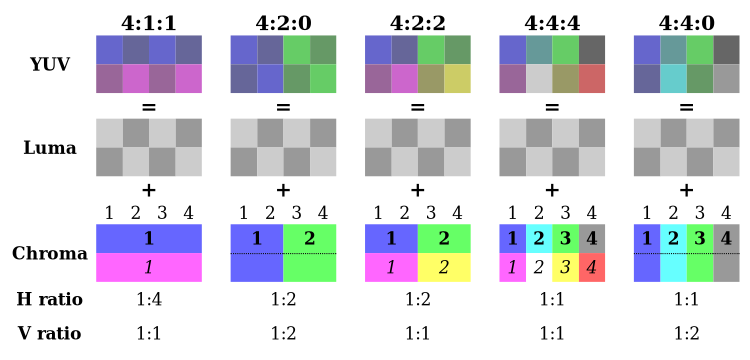
\includegraphics[width=0.55\textwidth]{slides/graphics-theory/yuv-sub-sampling.pdf}

  YUV 4:2:0 usual example:
  {\small
  \begin{equation*}
  \begin{gathered}
  bpp_Y = 8,~bpp_U = bpp_V = 8 \div 2 \div 2 = 2 \\
  \Rightarrow~ bpp = bpp_Y + bpp_U + bpp_V = 12~bits/pixel
  \end{gathered}
  \end{equation*}
  }
  \end{center}
\end{frame}

\begin{frame}{Pixel data distribution in memory}
  \begin{itemize}
  \item Pixel data can be \textbf{distributed} in different ways in memory
  \item Different ways to aggregate color components in \textbf{data planes} (memory chunks):
    \begin{itemize}
    \item \textbf{Packed}: Components are stored in the same data plane in memory
    \item \textbf{Semi-planar} (YUV): Luma and chroma are stored in distinct data planes
    \item \textbf{Planar}: Each component has its own data plane in memory
    \end{itemize}
  \item When multiple color components are grouped, \textbf{bit order} must be specified:
    \begin{itemize}
    \item Which component comes first in memory?
    \item Affected by endianness when read by hardware!
    \end{itemize}
  \item \textbf{Scan order} must also be specified:
    \begin{itemize}
    \item How to calculate the address for position \((x,y)\) and back?
    \item Raster order (most common) specifies: row-major, left-to-right, top-to-bottom
    \end{itemize}
  \end{itemize}
  \begin{center}
  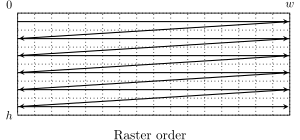
\includegraphics[height=6em]{slides/graphics-theory/raster-order.pdf}
  \end{center}
\end{frame}

\begin{frame}[fragile]{Pixel formats, FourCC codes}
  \begin{itemize}
  \item Many meta-data elements are needed to fully describe how a picture is coded
    \begin{itemize}
    \item Some describe \textbf{picture-level attributes} (e.g. dimensions)
    \item Some describe \textbf{pixel-level attributes} (e.g. colorspace, bpp)
    \end{itemize}
  \item Pixel-level attributes are grouped as a \textbf{pixel format} that defines:
    \begin{itemize}
    \item Colorspace in use
    \item Number of bits per channel and per pixel (bpp)
    \item Bit attribution and byte order
    \item Per-channel sub-sampling ratios
    \item Pixel data planes distribution in memory
    \end{itemize}
  \item Often represented as a 4-character code called \textbf{FourCC} {\small(\url{https://fourcc.org/})}\\
  \item Not really standardized and implementation-specific:\\
    \textit{DRM in Linux uses \code{XR24} for \ksym{DRM_FORMAT_XRGB8888}}.\\
  \textit{Not really standardized but widely used in various forms}
  \item Scan order is specified separately with a \textbf{modifier}\\
    \textit{Assumed to be raster order if unspecified}
  \end{itemize}
\end{frame}

\begin{frame}{Level of detail of quantized pictures}
  Depends on a number of factors, including:
  \begin{itemize}
  \item Spatial density (pixel resolution)
  \item Quantized dimensions (picture width and height)
  \item Colorspace limits (chromaticity diagram)
  \item Color depth (number of bits per pixel)
  \item Color resolution and range trade-off
  \end{itemize}~

  Generally speaking:
  \begin{itemize}
  \item Many factors are involved
  \item The major bottleneck is not always obvious
  \item Implementation choices do matter
  \end{itemize}
\end{frame}

\subsection{Pixel Drawing}

\begin{frame}{Accessing pixel data}
  \begin{itemize}
  \item Information required to access pixel data in memory:
    \begin{itemize}
    \item Pixel format (also modifier if not linear/raster order)
    \item Dimensions (and total size)
    \item Pointer to the base buffer address
    \end{itemize}
  \item The size of each line is called \textbf{stride} or \textbf{pitch}
    \begin{itemize}
    \item Usually equals: \(stride = width \times bpp \div 8\)
    \item Can contain an extra dead zone at the end
    \item Also needs to be specified explicitly
    \end{itemize}
  \item CPU access is either byte or word-aligned
    \begin{itemize}
    \item Good fit for formats with \(bpp = 32\) (very common)
    \item Good fit for formats with \(bpp = 8 \times n\)
    \item Not always easy to manage otherwise
    \end{itemize}
  \end{itemize}
\end{frame}

\begin{frame}[fragile]{Iterating over pixel data}
  \begin{itemize}
  \item Selected format (slides and demos): \textbf{XRGB8888}
    \begin{itemize}
    \item \(bpp = 32 = 8 \times 4\), one byte per channel, one memory plane
    \end{itemize}
  \item Pixel data can be access by iterating nested variables:
  \begin{minted}[fontsize=\small]{c}
for (y = 0; y < height; y++)
  for (x = 0; x < width; x++)
    data = base + y * stride + x * 4;
  \end{minted}
  \item Iterating over all pixels takes numerous CPU-cycles, tips:
    \begin{itemize}
    \item Incrementing the address instead of re-calculating it:
  \begin{minted}[fontsize=\small]{c}
data = base;
for (y = 0; y < height; y++)
  for (x = 0; x < width; x++)
    data += 4;
  data += stride - width * 4;
  \end{minted}
    \item Iterating in y-major is also better for cache hits
    \item Beware: C pointer arithmetic uses type size as unit
    \end{itemize}
  \end{itemize}
\end{frame}

\begin{frame}{Concepts about rasterization}
  \begin{itemize}
  \item Rasterization is the process of drawing vector shapes as discrete pixels
    \begin{itemize}
    \item Vector shapes are defined with mathematical equations
    \item Converted from a continuous space domain: \(\mathbb{R}^2\) to a discrete domain
    \item Results in a discretization/quantization error due to integer rounding
    \item Also subject to aliasing-related trouble
    \end{itemize}
  \end{itemize}
  \vspace{1em}
  \begin{minipage}[b]{0.45\textwidth}
    \centering
    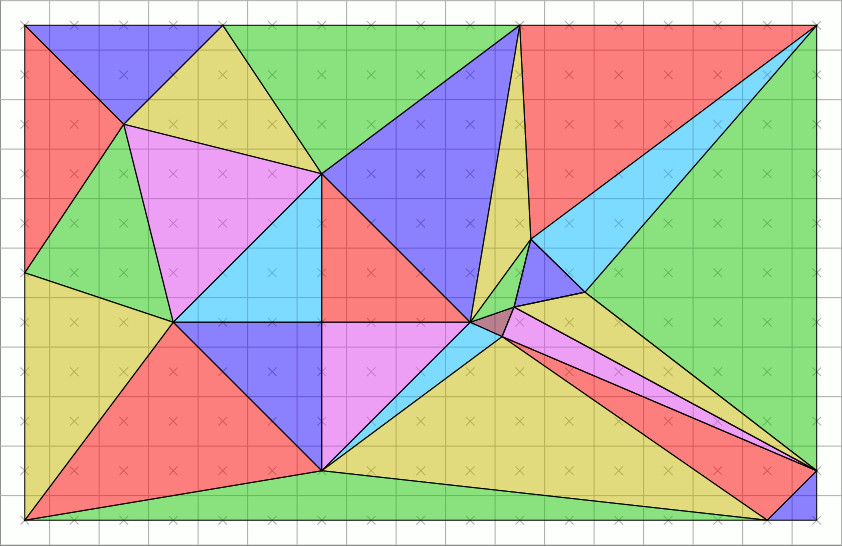
\includegraphics[width=0.8\textwidth]{slides/graphics-theory/raster-source.jpg}
    \textit{\small Continuous source representation}
  \end{minipage}
  \hfill
  \begin{minipage}[b]{0.45\textwidth}
    \centering
    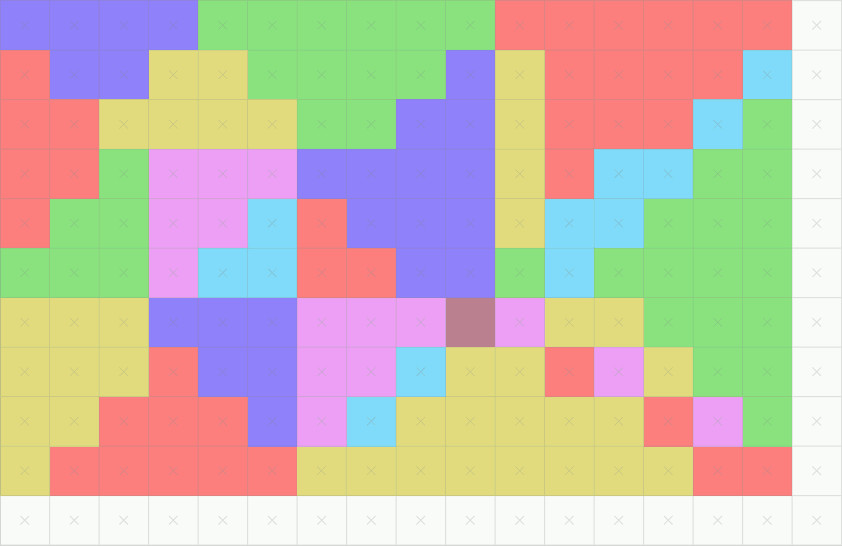
\includegraphics[width=0.8\textwidth]{slides/graphics-theory/raster-destination.jpg}
    \textit{\small Rasterized destination representation}
  \end{minipage}
\end{frame}

\begin{frame}{Rectangle drawing}
  \begin{itemize}
  \item A rectangle is defined with two boundaries per axis:
\[
x_{min} \leq x \leq x_{max},~ y_{min} \leq y \leq y_{max}
\]
  \item Another expression involves a (top-left) start point and size:
\[
x_{start} \leq x \leq x_{start} + x_{size},~ y_{start} \leq y \leq y_{start} + y_{size}
\]
  \item Allows iterating in the rectangle area only
  \end{itemize}
\end{frame}

\begin{frame}{Linear gradient drawing}
  \begin{itemize}
  \item Same base as drawing a rectangle
  \item A linear gradient involves interpolation between two colors
  \item Following one of the two axes as major
  \item Involves weighting the two colors depending on the advancement
  \item Equations in x-axis major:
  \end{itemize}
\begin{align*}
r &= r_{start} + (r_{stop} - r_{start}) \frac{x - x_{start}}{x_{size}}\\
g &= g_{start} + (g_{stop} - g_{start}) \frac{x - x_{start}}{x_{size}}\\
b &= b_{start} + (b_{stop} - b_{start}) \frac{x - x_{start}}{x_{size}}
\end{align*}
\end{frame}

\begin{frame}{Disk drawing}
  \begin{itemize}
  \item A disk is delimited with a radius test (\((0,0)\)-centered):
\[
\sqrt{x^2 + y^2} \leq radius
\]
  \item Given a center point \((x_c,y_c)\):
\[
\sqrt{(x - x_c)^2 + (y - y_c)^2} \leq radius
\]
  \item Requires iterating in:
\[
x_c - radius \leq x \leq x_c + radius,~ y_c - radius \leq y \leq y_c + radius
\]
  \end{itemize}
\end{frame}

\begin{frame}{Circular gradient drawing}
  \begin{itemize}
  \item Same base as drawing a disk
  \item Interpolation between two colors using the radius as major:
  \end{itemize}
\begin{align*}
d &= \sqrt{(x - x_c)^2 + (y - y_c)^2}\\
r &= r_{start} + (r_{stop} - r_{start}) \frac{d}{radius}\\
g &= g_{start} + (g_{stop} - g_{start}) \frac{d}{radius}\\
b &= b_{start} + (b_{stop} - b_{start}) \frac{d}{radius}
\end{align*}
\end{frame}

\begin{frame}{Line drawing}
  \begin{itemize}
  \item A line is defined as an affine function:
\[
y(x) = a \times x + b
\]
  \item Given start and end points, iterating in x-major:
\begin{gather*}
y(x) = y_{start} + (x - x_{start}) \times \frac{y_{end} - y_{start}}{x_{end} - x_{start}}\\
x_{start} \leq x \leq x_{stop}
\end{gather*}
  \item Axis major depends on the largest per-axis span (\(axis_{stop} - axis_{start}\))
    \begin{itemize}
    \item Iterating with smaller-span axis-major results in visual holes
    \item Iterating on both axes provides coherent results
    \end{itemize}
  \item Algorithms producing better-looking results:
    \begin{itemize}
    \item \textbf{Bresenham's} line algorithm, optimized for implementation
    \item \textbf{Xiaolin Wu's} line algorithm, with sub-pixel rendering
    \end{itemize}
  \end{itemize}
\end{frame}

\begin{frame}{Line and shape aliasing, sub-pixel drawing}
  \begin{itemize}
  \item Lines are often subject to aliasing:
    \begin{itemize}
    \item Sampled from the continuous domain with pixel sampling resolution
    \item Selecting the best axis gives a better resolution
    \item Limited display resolutions still make them look pixelated
    \end{itemize}
  \item Any geometric shape is affected, especially fonts
  \item Sub-pixel rendering is used to provide anti-aliased results:
    \begin{itemize}
    \item Surrounding pixels are given an intermediate value
    \item Specific algorithms perform sub-pixel drawing
    \item Also obtained with high-resolution rendering and anti-aliased downscaling
    \end{itemize}
  \end{itemize}

  \begin{center}
  
\includegraphics[height=4em]{slides/graphics-theory/diamond-sub-pixel.png}
  
\includegraphics[height=4em]{slides/graphics-theory/line-sub-pixel.png}\\
  \textit{\small Shapes rendered without and with sub-pixel anti-aliasing}
  \end{center}
\end{frame}

\begin{frame}{Line and shape aliasing, sub-pixel drawing (illustrated)}
  \begin{center}
  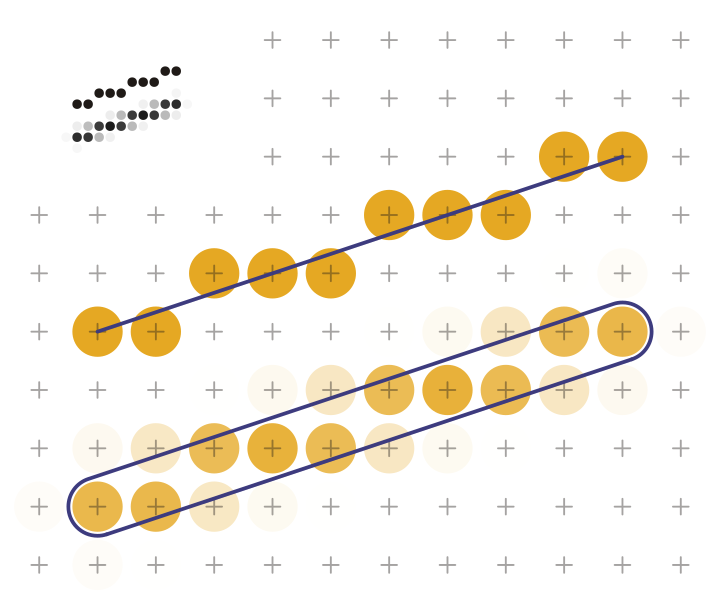
\includegraphics[width=0.4\textwidth]{slides/graphics-theory/line-sub-pixel-rendering.pdf}\\
  \textit{\small Pixel drawing versus sub-pixel drawing (x-axis major)}
  \end{center}
\end{frame}

\begin{frame}{Circles and polar coordinates}
  \begin{itemize}
  \item Circles centered on \((x_c,y_c)\) are defined (Pythagoras theorem) as:
\[
(x - x_c)^2+(y - y_c)^2 = radius^2
\]
  \end{itemize}
  \begin{minipage}{0.70\textwidth}
  \begin{itemize}
  \item Which is always verified with the expression:
\begin{gather*}
x = x_c + radius \times cos(\phi)\\
y = y_c + radius \times sin(\phi)
\end{gather*}
  \item Corresponds to a translation in polar coordinates
    \begin{itemize}
    \item From a \((x,y)\) base to \((r,\phi)\)
    \end{itemize}
  \item Iteration on \(\phi\) with a specific range: \(\phi \in [0;2\pi]\)
  \end{itemize}
  \end{minipage}
  \hfill
  \begin{minipage}{0.25\textwidth}
    \centering
    \includegraphics[width=0.8\textwidth]{slides/graphics-theory/polar-coordinates.pdf}
  \end{minipage}
\end{frame}

\begin{frame}{Parametric curves}
  \begin{itemize}
  \item Parametric curves generalize the idea of using independent parameters
  \item Each curve has defining equations and ranges for parameters
    \begin{itemize}
    \item Equations allow calculating \((x,y)\) (or \((r,\phi)\))
    \end{itemize}
  \item Drawing is achieved by iterating over parameter values
    \begin{itemize}
    \item Sampling is done on the range to get a finite number of points
    \item X/Y coordinates are calculated for each point
    \item Line interpolation is used between consecutive points
    \end{itemize}
  \item Ellipse: \(\phi \in [0;2\pi]\)
\begin{gather*}
x = x_c + a \times cos(\phi)\\
y = y_c + b \times sin(\phi)
\end{gather*}
  \item Many more parametric curves exist:
    \begin{itemize}
    \item Cycloid, Epicycloid, Epitrochoid, Hypocycloid, Hypotrochoid (spirograph)
    \item Lissajous Curve, Rose curve, Butterfly curve
    \end{itemize}
  \end{itemize}
\end{frame}

\subsection{Pixel Operations}

\begin{frame}{Region copy}
  \begin{itemize}
  \item Requirements for all pixel operations:
    \begin{itemize}
    \item The source and destination must use the same pixel format
    \item Must be converted before any operation otherwise
    \end{itemize}
  \item Most basic operation on pixels: copying a region
    \begin{itemize}
    \item Also known as bit blit or BITBLT (in reference to the hardware opcode)
    \end{itemize}
  \item Implemented as a line-per-line copy (maximum memory-contiguous block)
  \item Overwriting destination memory with source memory
    \begin{itemize}
    \item Copies within the same image are not always safe!
    \item Destination must not overlap source
    \end{itemize}
  \end{itemize}
\end{frame}

\begin{frame}{Alpha blending}
  \begin{itemize}
  \item Compositing multiple alpha-enabled pixel sources into a single result
    \begin{itemize}
    \item Simplest case: aggregating sources with z-ordered stacking
    \item Equation for A over B (with \(\alpha\) the alpha and \(C\) the color component value):
    \end{itemize}
\[
C_o = \frac{C_a \alpha_a + C_b \alpha_b \left(1 - \alpha_a\right)}{\alpha_a + \alpha_b \left(1 - \alpha_a\right)}
\]
  \item With alpha available, many more operations become possible
    \begin{itemize}
    \item Shapes can be used as masks, with logic operators
    \item Formalized by Porter and Duff in 1984
    \end{itemize}
  \end{itemize}
  \begin{center}
  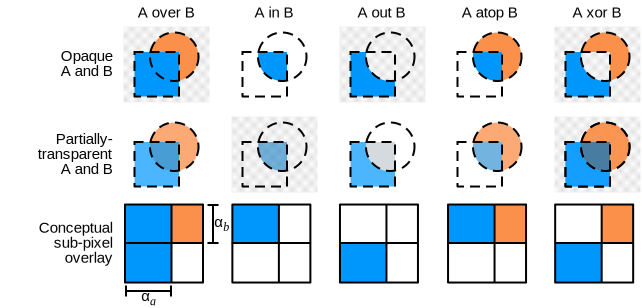
\includegraphics[width=0.5\textwidth]{slides/graphics-theory/porter-duff-compositing.pdf}
  \end{center}
\end{frame}

\begin{frame}{Color-keying}
  \begin{itemize}
  \item Color-keying (or chroma-keying): replacing given colors with alpha
  \item Specified with color ranges (3 RGB ranges)
  \item Pixels either within or outside of the range are made transparent
  \item Used in conjunction with alpha blending
  \item The famous video green-screen method uses color-keying
  \end{itemize}
  \begin{center}
  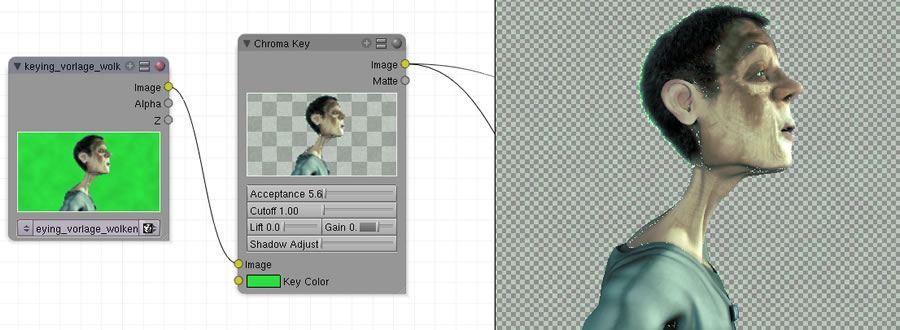
\includegraphics[width=0.5\textwidth]{slides/graphics-theory/chroma-key-blender.jpg}\\
  \textit{\small Color-keying implemented in Blender}
  \end{center}
\end{frame}

\begin{frame}{Scaling and interpolation}
  \begin{itemize}
  \item Scaling is a resizing operation on a pixel picture
    \begin{itemize}
    \item Involves a scaling factor (integer or real)
    \item Values are resampled with a new resolution
    \item Requires reconstructing the original signal
    \end{itemize}
  \item Implemented with some form of interpolation:
    \begin{itemize}
    \item nearest-neighbor: uses the nearest pixel value from the source
\[
x_{source} = x_{destination} \times scale
\]
  \item bilinear interpolation: sub-pixel linear weighting of neighbor colors
  \item bicubic interpolation: smooth spline sub-pixel fitting with neighbor colors
    \end{itemize}
  \item Sub-pixel methods provide better visual results
  \item Down-sampling:
    \begin{itemize}
    \item Reduces the maximum image frequency
    \item Can cause aliasing: high frequencies need to be removed
    \end{itemize}
  \end{itemize}
\end{frame}

\begin{frame}{Linear filtering and convolution}
  \begin{itemize}
  \item Filtering is a transformation of each pixel based on its neighbors
  \item The pixel output value is a linear sum of weighted neighboring input values
\[
o_{x,y} = \alpha_0 i_{x,y} + \alpha_1 i_{x-1,y} + \alpha_2 i_{x+1,y} + ...
\]
  \item Weighting coefficients are represented in a 2D matrix: the \textbf{filter kernel}
    \begin{itemize}
    \item Comes with \(2n + 1\) columns and \(2m + 1\) rows
    \item The coefficients are applied to each input pixel and its neighbors
    \item The element at the kernel center weights the current input pixel
    \end{itemize}
  \item Corresponds to a \textbf{convolution} operation between pixels and the filter kernel
  \item High computational cost (optimizations are implemented)
  \item Allows many applications for 2D signal processing
  \end{itemize}
\end{frame}

\begin{frame}{Linear filtering and convolution (illustrated)}
  \begin{center}
  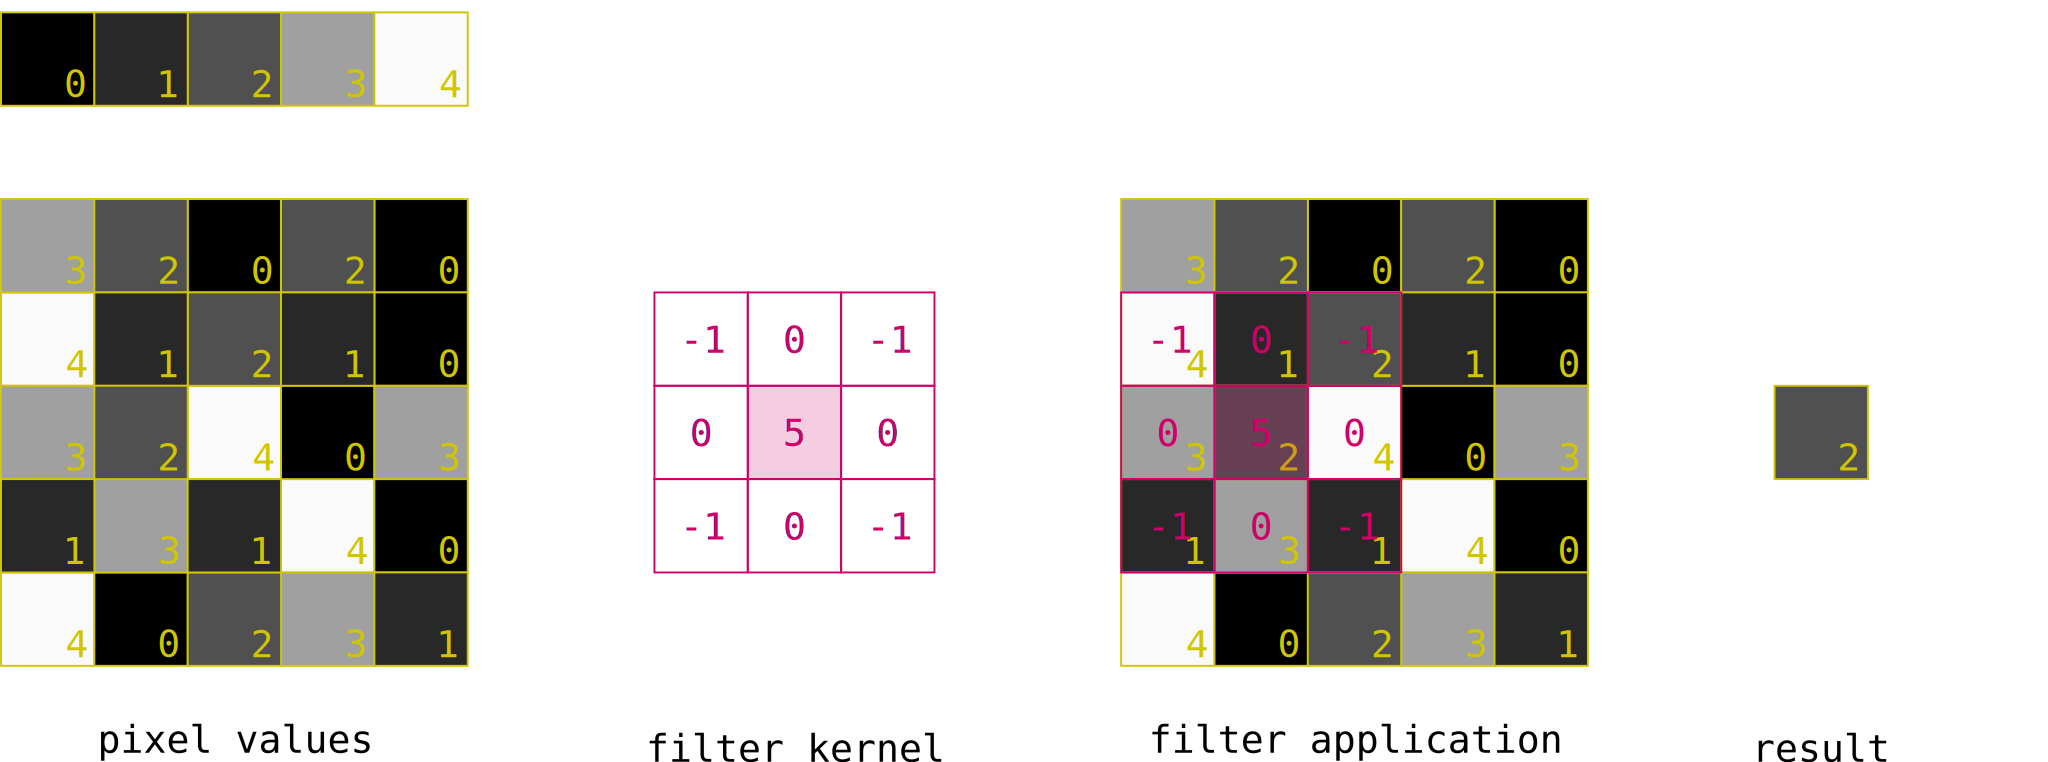
\includegraphics[width=0.7\textwidth]{slides/graphics-theory/linear-filtering.pdf}\\
  \textit{\small Linear filtering in application}
\[
g(x,y)= \omega *f(x,y)=\sum_{s=-n}^n{\sum_{t=-m}^m{ \omega (s,t)f(x-s,y-t)}}
\]
  \textit{\small Bi-dimensional convolution operation on \(f\) with the \(\omega\) kernel}
  \end{center}
\end{frame}

\begin{frame}{Blur filters}
  \begin{itemize}
  \item Blurring is a common example of linear filtering
  \item Corresponds to a low-pass filter
    \begin{itemize}
    \item Removes high frequencies from the picture (details)
    \item Good fit for pre-scaling anti-aliasing
    \end{itemize}
\begin{minipage}[b]{0.45\textwidth}
  \item Implemented with different algorithms:
    \vspace{-1.5em}
    \begin{itemize}
    \item Box blur: rough but easy to optimize
\[
\frac{1}{9}
\left[
\begin{matrix}
1 & 1 & 1 \\
1 & 1 & 1 \\
1 & 1 & 1
\end{matrix}
\right]
\]
    \end{itemize}
\end{minipage}
\begin{minipage}[b]{0.45\textwidth}
    \begin{itemize}
    \item Gaussian blur: reference smooth blur
\[
\frac{1}{16}
\left[
\begin{matrix}
1 & 2 & 1 \\
2 & 4 & 2 \\
1 & 2 & 1
\end{matrix}
\right]
\]
    \end{itemize}
    \end{minipage}
  \item A repeated box blur converges towards a Gaussian one (central-limit theorem)
  \end{itemize}
\end{frame}

\begin{frame}{Dithering}
  \begin{itemize}
  \item Reducing the color depth can lead to visually-unpleasant results
    \begin{itemize}
    \item Corresponds to color-space down-sampling
    \item Increases color quantization error
    \end{itemize}
  \item Floyd–Steinberg dithering is a method for improving quality with low depth
  \item Quantization error is evaluated and distributed to neighboring pixels
  \item Used in hardware display engines and the GIF file format
  \end{itemize}~\\

  \begin{minipage}[t]{0.25\textwidth}
    \centering
    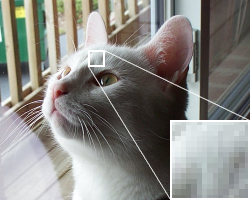
\includegraphics[width=0.9\textwidth]{slides/graphics-theory/cat-depth-initial.png}\\
    \textit{\small Cat at initial depth}
  \end{minipage}
  \hfill
  \begin{minipage}[t]{0.25\textwidth}
    \centering
    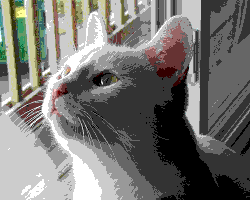
\includegraphics[width=0.9\textwidth]{slides/graphics-theory/cat-depth-low.png}\\
    \textit{\small Cat at reduced depth without dithering}
  \end{minipage}
  \hfill
  \begin{minipage}[t]{0.25\textwidth}
    \centering
    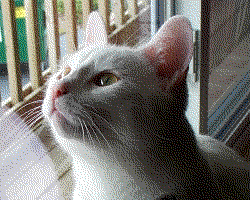
\includegraphics[width=0.9\textwidth]{slides/graphics-theory/cat-depth-dither.png}\\
    \textit{\small Cat at reduced depth with dithering}
  \end{minipage}
\end{frame}

\begin{frame}{Graphics theory online references}
  \small
  \begin{itemize}
  \item Wikipedia (\url{https://en.wikipedia.org/}):
    \begin{itemize}
    \item \href{https://en.wikipedia.org/wiki/Color_model}{Color model}
    \item \href{https://en.wikipedia.org/wiki/Color_depth}{Color depth}
    \item \href{https://en.wikipedia.org/wiki/YCbCr}{YCbCr}
    \item \href{https://en.wikipedia.org/wiki/Chroma_subsampling}{Chroma subsampling}
    \item \href{https://en.wikipedia.org/wiki/Nyquist–Shannon_sampling_theorem}{Nyquist–Shannon sampling theorem}
    \item \href{https://en.wikipedia.org/wiki/Spatial_anti-aliasing}{Spatial anti-aliasing}
    \item \href{https://en.wikipedia.org/wiki/Aliasing}{Aliasing}
    \item \href{https://en.wikipedia.org/wiki/Line_drawing_algorithm}{Line drawing algorithm}
    \item \href{https://en.wikipedia.org/wiki/Parametric_equation}{Parametric equation}
    \item \href{https://en.wikipedia.org/wiki/Alpha_compositing}{Alpha compositing}
    \item \href{https://en.wikipedia.org/wiki/Image_scaling}{Image scaling}
    \item \href{https://en.wikipedia.org/wiki/Kernel_(image_processing)}{Kernel (image processing)}
    \end{itemize}
  \item \url{http://ssp.impulsetrain.com/porterduff.html}
  \item \url{https://magcius.github.io/xplain/article/regions.html}
  \item \url{https://magcius.github.io/xplain/article/rast1.html}
  \end{itemize}
\end{frame}

\begin{frame}{Graphics theory illustrations attributions}
  \small
  \begin{itemize}
  \item \href{https://commons.wikimedia.org/wiki/File:2017-12-28_Leipzig,_34c3,_Fairy_Dust_(freddy2001).jpg}{34C3 Fairy Dust: Freddy2001, CC BY-SA 3.0}
  \item \href{https://commons.wikimedia.org/wiki/File:View_from_the_Window_at_Le_Gras,_Joseph_Nic\%C3\%A9phore_Ni\%C3\%A9pce.jpg}{Point de vue du Gras: Joseph Nicéphore Niépce, public domain}
  \item \href{https://commons.wikimedia.org/wiki/File:Pinball_Dot_Matrix_Display_-_Demolition_Man.JPG}{Pinball Dot Matrix Display: ElHeineken, CC BY 3.0}
  \item \href{https://commons.wikimedia.org/wiki/File:Soderledskyrkan_brick_wall.jpg}{Soderledskyrkan brick wall: Xauxa, CC BY-SA 3.0}
  \item \href{https://commons.wikimedia.org/wiki/File:AliasingSines.svg}{Aliasing Sines: Moxfyre, CC BY-SA 3.0}
  \item \href{https://commons.wikimedia.org/wiki/File:Moire_pattern_of_bricks.jpg}{Moiré pattern of bricks: Colin M.L. Burnett, CC BY-SA 3.0}
  \item \href{https://commons.wikimedia.org/wiki/File:Moire_pattern_of_bricks_small.jpg}{Moiré Pattern at Gardham Gap: Roger Gilbertson, CC BY-SA 2.0}
  \item \href{https://commons.wikimedia.org/wiki/File:RGBCube_a.svg}{RGB cube: Datumizer, CC BY-SA 4.0}
  \item \href{https://commons.wikimedia.org/wiki/File:Pair_of_Merops_apiaster_feeding.jpg}{Pair of Merops apiaster feeding: Pierre Dalous, CC BY-SA 3.0}
  \end{itemize}
\end{frame}

\begin{frame}{Graphics theory illustrations attributions}
  \small
  \begin{itemize}
  \item \href{https://commons.wikimedia.org/wiki/File:Hsl-hsv_models_b.svg}{Hsl-hsv models: Datumizer, CC BY-SA 3.0}
  \item \href{https://commons.wikimedia.org/wiki/File:Barns_grand_tetons.jpg}{Barns grand tetons: Jon Sullivan, public domain}
  \item \href{https://commons.wikimedia.org/wiki/File:Top-left_triangle_rasterization_rule.gif}{Top-left triangle rasterization rule: Drummyfish, CC0 1.0}
  \item \href{https://commons.wikimedia.org/wiki/File:Line_scan-conversion.svg}{Line scan-conversion: Phrood, CC BY-SA 3.0}
  \item \href{https://commons.wikimedia.org/wiki/File:Alpha_compositing.svg}{Alpha compositing: Prometeusm, Wereon, public domain}
  \item \href{https://commons.wikimedia.org/wiki/File:Blender3D_com_key_chroma.jpg}{Blender3D com key chroma: Toni Grappa, Blender Foundation, CC BY-2.5}
  \item \href{https://en.wikipedia.org/wiki/File:Dithering_example_dithered_web_palette.png}{Dithering example: Jamelan, CC BY-SA 3.0}
  \end{itemize}
\end{frame}
